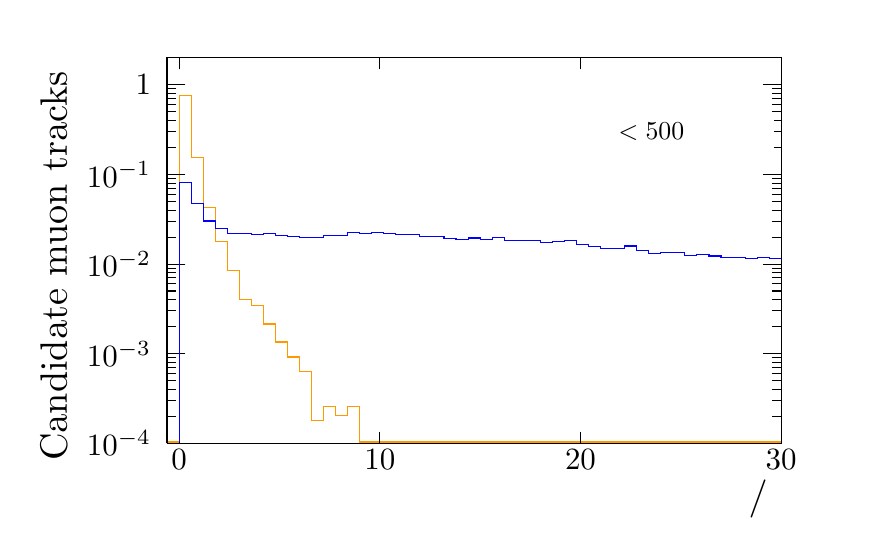
\begin{tikzpicture}
\pgfdeclareplotmark{cross} {
\pgfpathmoveto{\pgfpoint{-0.3\pgfplotmarksize}{\pgfplotmarksize}}
\pgfpathlineto{\pgfpoint{+0.3\pgfplotmarksize}{\pgfplotmarksize}}
\pgfpathlineto{\pgfpoint{+0.3\pgfplotmarksize}{0.3\pgfplotmarksize}}
\pgfpathlineto{\pgfpoint{+1\pgfplotmarksize}{0.3\pgfplotmarksize}}
\pgfpathlineto{\pgfpoint{+1\pgfplotmarksize}{-0.3\pgfplotmarksize}}
\pgfpathlineto{\pgfpoint{+0.3\pgfplotmarksize}{-0.3\pgfplotmarksize}}
\pgfpathlineto{\pgfpoint{+0.3\pgfplotmarksize}{-1.\pgfplotmarksize}}
\pgfpathlineto{\pgfpoint{-0.3\pgfplotmarksize}{-1.\pgfplotmarksize}}
\pgfpathlineto{\pgfpoint{-0.3\pgfplotmarksize}{-0.3\pgfplotmarksize}}
\pgfpathlineto{\pgfpoint{-1.\pgfplotmarksize}{-0.3\pgfplotmarksize}}
\pgfpathlineto{\pgfpoint{-1.\pgfplotmarksize}{0.3\pgfplotmarksize}}
\pgfpathlineto{\pgfpoint{-0.3\pgfplotmarksize}{0.3\pgfplotmarksize}}
\pgfpathclose
\pgfusepathqstroke
}
\pgfdeclareplotmark{cross*} {
\pgfpathmoveto{\pgfpoint{-0.3\pgfplotmarksize}{\pgfplotmarksize}}
\pgfpathlineto{\pgfpoint{+0.3\pgfplotmarksize}{\pgfplotmarksize}}
\pgfpathlineto{\pgfpoint{+0.3\pgfplotmarksize}{0.3\pgfplotmarksize}}
\pgfpathlineto{\pgfpoint{+1\pgfplotmarksize}{0.3\pgfplotmarksize}}
\pgfpathlineto{\pgfpoint{+1\pgfplotmarksize}{-0.3\pgfplotmarksize}}
\pgfpathlineto{\pgfpoint{+0.3\pgfplotmarksize}{-0.3\pgfplotmarksize}}
\pgfpathlineto{\pgfpoint{+0.3\pgfplotmarksize}{-1.\pgfplotmarksize}}
\pgfpathlineto{\pgfpoint{-0.3\pgfplotmarksize}{-1.\pgfplotmarksize}}
\pgfpathlineto{\pgfpoint{-0.3\pgfplotmarksize}{-0.3\pgfplotmarksize}}
\pgfpathlineto{\pgfpoint{-1.\pgfplotmarksize}{-0.3\pgfplotmarksize}}
\pgfpathlineto{\pgfpoint{-1.\pgfplotmarksize}{0.3\pgfplotmarksize}}
\pgfpathlineto{\pgfpoint{-0.3\pgfplotmarksize}{0.3\pgfplotmarksize}}
\pgfpathclose
\pgfusepathqfillstroke
}
\pgfdeclareplotmark{newstar} {
\pgfpathmoveto{\pgfqpoint{0pt}{\pgfplotmarksize}}
\pgfpathlineto{\pgfqpointpolar{44}{0.5\pgfplotmarksize}}
\pgfpathlineto{\pgfqpointpolar{18}{\pgfplotmarksize}}
\pgfpathlineto{\pgfqpointpolar{-20}{0.5\pgfplotmarksize}}
\pgfpathlineto{\pgfqpointpolar{-54}{\pgfplotmarksize}}
\pgfpathlineto{\pgfqpointpolar{-90}{0.5\pgfplotmarksize}}
\pgfpathlineto{\pgfqpointpolar{234}{\pgfplotmarksize}}
\pgfpathlineto{\pgfqpointpolar{198}{0.5\pgfplotmarksize}}
\pgfpathlineto{\pgfqpointpolar{162}{\pgfplotmarksize}}
\pgfpathlineto{\pgfqpointpolar{134}{0.5\pgfplotmarksize}}
\pgfpathclose
\pgfusepathqstroke
}
\pgfdeclareplotmark{newstar*} {
\pgfpathmoveto{\pgfqpoint{0pt}{\pgfplotmarksize}}
\pgfpathlineto{\pgfqpointpolar{44}{0.5\pgfplotmarksize}}
\pgfpathlineto{\pgfqpointpolar{18}{\pgfplotmarksize}}
\pgfpathlineto{\pgfqpointpolar{-20}{0.5\pgfplotmarksize}}
\pgfpathlineto{\pgfqpointpolar{-54}{\pgfplotmarksize}}
\pgfpathlineto{\pgfqpointpolar{-90}{0.5\pgfplotmarksize}}
\pgfpathlineto{\pgfqpointpolar{234}{\pgfplotmarksize}}
\pgfpathlineto{\pgfqpointpolar{198}{0.5\pgfplotmarksize}}
\pgfpathlineto{\pgfqpointpolar{162}{\pgfplotmarksize}}
\pgfpathlineto{\pgfqpointpolar{134}{0.5\pgfplotmarksize}}
\pgfpathclose
\pgfusepathqfillstroke
}
\definecolor{c}{rgb}{1,1,1};
\draw [color=c, fill=c] (0,0) rectangle (10,6.27517);
\draw [color=c, fill=c] (1.4,1.00403) rectangle (9.2,5.89866);
\definecolor{c}{rgb}{0,0,0};
\draw [c] (1.4,1.00403) -- (1.4,5.89866) -- (9.2,5.89866) -- (9.2,1.00403) -- (1.4,1.00403);
\definecolor{c}{rgb}{1,1,1};
\draw [color=c, fill=c] (1.4,1.00403) rectangle (9.2,5.89866);
\definecolor{c}{rgb}{0,0,0};
\draw [c] (1.4,1.00403) -- (1.4,5.89866) -- (9.2,5.89866) -- (9.2,1.00403) -- (1.4,1.00403);
\definecolor{c}{rgb}{1,0.6,0};
\draw [c,line width=0.4] (1.41678,1.02081) -- (1.41678,1.02081) -- (1.55294,1.02081) -- (1.55294,5.42255) -- (1.70588,5.42255) -- (1.70588,4.62973) -- (1.85882,4.62973) -- (1.85882,4.00033) -- (2.01176,4.00033) -- (2.01176,3.56618) --
 (2.16471,3.56618) -- (2.16471,3.20048) -- (2.31765,3.20048) -- (2.31765,2.83364) -- (2.47059,2.83364) -- (2.47059,2.75277) -- (2.62353,2.75277) -- (2.62353,2.51827) -- (2.77647,2.51827) -- (2.77647,2.29067) -- (2.92941,2.29067) -- (2.92941,2.09951)
 -- (3.08235,2.09951) -- (3.08235,1.91929) -- (3.23529,1.91929) -- (3.23529,1.29015) -- (3.38824,1.29015) -- (3.38824,1.46643) -- (3.54118,1.46643) -- (3.54118,1.35615) -- (3.69412,1.35615) -- (3.69412,1.46643) -- (3.84706,1.46643) --
 (3.84706,1.02081) -- (4,1.02081) -- (4,1.02081) -- (4.15294,1.02081) -- (4.15294,1.02081) -- (4.30588,1.02081) -- (4.30588,1.02081) -- (4.45882,1.02081) -- (4.45882,1.02081) -- (4.61176,1.02081) -- (4.61176,1.02081) -- (4.76471,1.02081) --
 (4.76471,1.02081) -- (4.91765,1.02081) -- (4.91765,1.02081) -- (5.07059,1.02081) -- (5.07059,1.02081) -- (5.22353,1.02081) -- (5.22353,1.02081) -- (5.37647,1.02081) -- (5.37647,1.02081) -- (5.52941,1.02081) -- (5.52941,1.02081) -- (5.68235,1.02081)
 -- (5.68235,1.02081) -- (5.83529,1.02081) -- (5.83529,1.02081) -- (5.98824,1.02081) -- (5.98824,1.02081) -- (6.14118,1.02081) -- (6.14118,1.02081) -- (6.29412,1.02081) -- (6.29412,1.02081) -- (6.44706,1.02081) -- (6.44706,1.02081) -- (6.6,1.02081)
 -- (6.6,1.02081) -- (6.75294,1.02081) -- (6.75294,1.02081) -- (6.90588,1.02081) -- (6.90588,1.02081) -- (7.05882,1.02081) -- (7.05882,1.02081) -- (7.21176,1.02081) -- (7.21176,1.02081) -- (7.36471,1.02081) -- (7.36471,1.02081) -- (7.51765,1.02081)
 -- (7.51765,1.02081) -- (7.67059,1.02081) -- (7.67059,1.02081) -- (7.82353,1.02081) -- (7.82353,1.02081) -- (7.97647,1.02081) -- (7.97647,1.02081) -- (8.12941,1.02081) -- (8.12941,1.02081) -- (8.28235,1.02081) -- (8.28235,1.02081) --
 (8.43529,1.02081) -- (8.43529,1.02081) -- (8.58823,1.02081) -- (8.58823,1.02081) -- (8.74118,1.02081) -- (8.74118,1.02081) -- (8.89412,1.02081) -- (8.89412,1.02081) -- (9.04706,1.02081) -- (9.04706,1.02081) -- (9.2,1.02081) -- (9.2,1.02081);
\definecolor{c}{rgb}{0,0,0};
\draw [c,line width=0.4] (1.4,1.00403) -- (9.2,1.00403);
\draw [anchor= east] (9.2,0.301208) node[scale=1.37879, rotate=0]{$\chisq/\nDoF$};
\draw [c,line width=0.4] (1.55294,1.15087) -- (1.55294,1.00403);
\draw [c,line width=0.4] (4.10196,1.15087) -- (4.10196,1.00403);
\draw [c,line width=0.4] (6.65098,1.15087) -- (6.65098,1.00403);
\draw [c,line width=0.4] (9.2,1.15087) -- (9.2,1.00403);
\draw [c,line width=0.4] (1.55294,1.15087) -- (1.55294,1.00403);
\draw [anchor=base] (1.55294,0.665168) node[scale=1.11794, rotate=0]{0};
\draw [anchor=base] (4.10196,0.665168) node[scale=1.11794, rotate=0]{10};
\draw [anchor=base] (6.65098,0.665168) node[scale=1.11794, rotate=0]{20};
\draw [anchor=base] (9.2,0.665168) node[scale=1.11794, rotate=0]{30};
\draw [c,line width=0.4] (1.4,5.89866) -- (9.2,5.89866);
\draw [c,line width=0.4] (1.55294,5.75182) -- (1.55294,5.89866);
\draw [c,line width=0.4] (4.10196,5.75182) -- (4.10196,5.89866);
\draw [c,line width=0.4] (6.65098,5.75182) -- (6.65098,5.89866);
\draw [c,line width=0.4] (9.2,5.75182) -- (9.2,5.89866);
\draw [c,line width=0.4] (1.55294,5.75182) -- (1.55294,5.89866);
\draw [c,line width=0.4] (1.4,1.00403) -- (1.4,5.89866);
\draw [anchor= east] (-0.04,5.89866) node[scale=1.37879, rotate=90]{Candidate muon tracks};
\draw [c,line width=0.4] (1.634,1.00403) -- (1.4,1.00403);
\draw [anchor= east] (1.336,1.00403) node[scale=1.11794, rotate=0]{$10^{-4}$};
\draw [c,line width=0.4] (1.517,1.3466) -- (1.4,1.3466);
\draw [c,line width=0.4] (1.517,1.547) -- (1.4,1.547);
\draw [c,line width=0.4] (1.517,1.68918) -- (1.4,1.68918);
\draw [c,line width=0.4] (1.517,1.79947) -- (1.4,1.79947);
\draw [c,line width=0.4] (1.517,1.88957) -- (1.4,1.88957);
\draw [c,line width=0.4] (1.517,1.96576) -- (1.4,1.96576);
\draw [c,line width=0.4] (1.517,2.03176) -- (1.4,2.03176);
\draw [c,line width=0.4] (1.517,2.08997) -- (1.4,2.08997);
\draw [c,line width=0.4] (1.634,2.14204) -- (1.4,2.14204);
\draw [anchor= east] (1.336,2.14204) node[scale=1.11794, rotate=0]{$10^{-3}$};
\draw [c,line width=0.4] (1.517,2.48462) -- (1.4,2.48462);
\draw [c,line width=0.4] (1.517,2.68501) -- (1.4,2.68501);
\draw [c,line width=0.4] (1.517,2.82719) -- (1.4,2.82719);
\draw [c,line width=0.4] (1.517,2.93748) -- (1.4,2.93748);
\draw [c,line width=0.4] (1.517,3.02759) -- (1.4,3.02759);
\draw [c,line width=0.4] (1.517,3.10377) -- (1.4,3.10377);
\draw [c,line width=0.4] (1.517,3.16977) -- (1.4,3.16977);
\draw [c,line width=0.4] (1.517,3.22798) -- (1.4,3.22798);
\draw [c,line width=0.4] (1.634,3.28005) -- (1.4,3.28005);
\draw [anchor= east] (1.336,3.28005) node[scale=1.11794, rotate=0]{$10^{-2}$};
\draw [c,line width=0.4] (1.517,3.62263) -- (1.4,3.62263);
\draw [c,line width=0.4] (1.517,3.82303) -- (1.4,3.82303);
\draw [c,line width=0.4] (1.517,3.96521) -- (1.4,3.96521);
\draw [c,line width=0.4] (1.517,4.07549) -- (1.4,4.07549);
\draw [c,line width=0.4] (1.517,4.1656) -- (1.4,4.1656);
\draw [c,line width=0.4] (1.517,4.24179) -- (1.4,4.24179);
\draw [c,line width=0.4] (1.517,4.30778) -- (1.4,4.30778);
\draw [c,line width=0.4] (1.517,4.366) -- (1.4,4.366);
\draw [c,line width=0.4] (1.634,4.41807) -- (1.4,4.41807);
\draw [anchor= east] (1.336,4.41807) node[scale=1.11794, rotate=0]{$10^{-1}$};
\draw [c,line width=0.4] (1.517,4.76064) -- (1.4,4.76064);
\draw [c,line width=0.4] (1.517,4.96104) -- (1.4,4.96104);
\draw [c,line width=0.4] (1.517,5.10322) -- (1.4,5.10322);
\draw [c,line width=0.4] (1.517,5.21351) -- (1.4,5.21351);
\draw [c,line width=0.4] (1.517,5.30361) -- (1.4,5.30361);
\draw [c,line width=0.4] (1.517,5.3798) -- (1.4,5.3798);
\draw [c,line width=0.4] (1.517,5.4458) -- (1.4,5.4458);
\draw [c,line width=0.4] (1.517,5.50401) -- (1.4,5.50401);
\draw [c,line width=0.4] (1.634,5.55608) -- (1.4,5.55608);
\draw [anchor= east] (1.336,5.55608) node[scale=1.11794, rotate=0]{1};
\draw [c,line width=0.4] (1.517,5.89866) -- (1.4,5.89866);
\draw [c,line width=0.4] (9.2,1.00403) -- (9.2,5.89866);
\draw [c,line width=0.4] (8.966,1.00403) -- (9.2,1.00403);
\draw [c,line width=0.4] (9.083,1.3466) -- (9.2,1.3466);
\draw [c,line width=0.4] (9.083,1.547) -- (9.2,1.547);
\draw [c,line width=0.4] (9.083,1.68918) -- (9.2,1.68918);
\draw [c,line width=0.4] (9.083,1.79947) -- (9.2,1.79947);
\draw [c,line width=0.4] (9.083,1.88957) -- (9.2,1.88957);
\draw [c,line width=0.4] (9.083,1.96576) -- (9.2,1.96576);
\draw [c,line width=0.4] (9.083,2.03176) -- (9.2,2.03176);
\draw [c,line width=0.4] (9.083,2.08997) -- (9.2,2.08997);
\draw [c,line width=0.4] (8.966,2.14204) -- (9.2,2.14204);
\draw [c,line width=0.4] (9.083,2.48462) -- (9.2,2.48462);
\draw [c,line width=0.4] (9.083,2.68501) -- (9.2,2.68501);
\draw [c,line width=0.4] (9.083,2.82719) -- (9.2,2.82719);
\draw [c,line width=0.4] (9.083,2.93748) -- (9.2,2.93748);
\draw [c,line width=0.4] (9.083,3.02759) -- (9.2,3.02759);
\draw [c,line width=0.4] (9.083,3.10377) -- (9.2,3.10377);
\draw [c,line width=0.4] (9.083,3.16977) -- (9.2,3.16977);
\draw [c,line width=0.4] (9.083,3.22798) -- (9.2,3.22798);
\draw [c,line width=0.4] (8.966,3.28005) -- (9.2,3.28005);
\draw [c,line width=0.4] (9.083,3.62263) -- (9.2,3.62263);
\draw [c,line width=0.4] (9.083,3.82303) -- (9.2,3.82303);
\draw [c,line width=0.4] (9.083,3.96521) -- (9.2,3.96521);
\draw [c,line width=0.4] (9.083,4.07549) -- (9.2,4.07549);
\draw [c,line width=0.4] (9.083,4.1656) -- (9.2,4.1656);
\draw [c,line width=0.4] (9.083,4.24179) -- (9.2,4.24179);
\draw [c,line width=0.4] (9.083,4.30778) -- (9.2,4.30778);
\draw [c,line width=0.4] (9.083,4.366) -- (9.2,4.366);
\draw [c,line width=0.4] (8.966,4.41807) -- (9.2,4.41807);
\draw [c,line width=0.4] (9.083,4.76064) -- (9.2,4.76064);
\draw [c,line width=0.4] (9.083,4.96104) -- (9.2,4.96104);
\draw [c,line width=0.4] (9.083,5.10322) -- (9.2,5.10322);
\draw [c,line width=0.4] (9.083,5.21351) -- (9.2,5.21351);
\draw [c,line width=0.4] (9.083,5.30361) -- (9.2,5.30361);
\draw [c,line width=0.4] (9.083,5.3798) -- (9.2,5.3798);
\draw [c,line width=0.4] (9.083,5.4458) -- (9.2,5.4458);
\draw [c,line width=0.4] (9.083,5.50401) -- (9.2,5.50401);
\draw [c,line width=0.4] (8.966,5.55608) -- (9.2,5.55608);
\draw [c,line width=0.4] (9.083,5.89866) -- (9.2,5.89866);
\definecolor{c}{rgb}{0,0,1};
\draw [c,line width=0.4] (1.55294,1.02081) -- (1.55294,4.31946) -- (1.70588,4.31946) -- (1.70588,4.04993) -- (1.85882,4.04993) -- (1.85882,3.82753) -- (2.01176,3.82753) -- (2.01176,3.73489) -- (2.16471,3.73489) -- (2.16471,3.6723) -- (2.31765,3.6723)
 -- (2.31765,3.66634) -- (2.47059,3.66634) -- (2.47059,3.65572) -- (2.62353,3.65572) -- (2.62353,3.66634) -- (2.77647,3.66634) -- (2.77647,3.64067) -- (2.92941,3.64067) -- (2.92941,3.63056) -- (3.08235,3.63056) -- (3.08235,3.61748) --
 (3.23529,3.61748) -- (3.23529,3.61526) -- (3.38824,3.61526) -- (3.38824,3.64434) -- (3.54118,3.64434) -- (3.54118,3.64747) -- (3.69412,3.64747) -- (3.69412,3.68451) -- (3.84706,3.68451) -- (3.84706,3.6723) -- (4,3.6723) -- (4,3.68451) --
 (4.15294,3.68451) -- (4.15294,3.6723) -- (4.30588,3.6723) -- (4.30588,3.65979) -- (4.45882,3.65979) -- (4.45882,3.65006) -- (4.61176,3.65006) -- (4.61176,3.62569) -- (4.76471,3.62569) -- (4.76471,3.62948) -- (4.91765,3.62948) -- (4.91765,3.60631) --
 (5.07059,3.60631) -- (5.07059,3.5943) -- (5.22353,3.5943) -- (5.22353,3.61137) -- (5.37647,3.61137) -- (5.37647,3.58789) -- (5.52941,3.58789) -- (5.52941,3.61526) -- (5.68235,3.61526) -- (5.68235,3.5814) -- (5.83529,3.5814) -- (5.83529,3.5814) --
 (5.98824,3.5814) -- (5.98824,3.57783) -- (6.14118,3.57783) -- (6.14118,3.55014) -- (6.29412,3.55014) -- (6.29412,3.56816) -- (6.44706,3.56816) -- (6.44706,3.57723) -- (6.6,3.57723) -- (6.6,3.53078) -- (6.75294,3.53078) -- (6.75294,3.50788) --
 (6.90588,3.50788) -- (6.90588,3.47732) -- (7.05882,3.47732) -- (7.05882,3.48024) -- (7.21176,3.48024) -- (7.21176,3.50926) -- (7.36471,3.50926) -- (7.36471,3.45251) -- (7.51765,3.45251) -- (7.51765,3.41404) -- (7.67059,3.41404) -- (7.67059,3.42882)
 -- (7.82353,3.42882) -- (7.82353,3.42312) -- (7.97647,3.42312) -- (7.97647,3.38397) -- (8.12941,3.38397) -- (8.12941,3.3988) -- (8.28235,3.3988) -- (8.28235,3.3822) -- (8.43529,3.3822) -- (8.43529,3.36132) -- (8.58823,3.36132) -- (8.58823,3.36317)
 -- (8.74118,3.36317) -- (8.74118,3.35195) -- (8.89412,3.35195) -- (8.89412,3.36501) -- (9.04706,3.36501) -- (9.04706,3.3453) -- (9.2,3.3453);
\definecolor{c}{rgb}{1,1,1};
\draw [color=c, fill=c] (6,4.70638) rectangle (9.1,5.20839);
\draw (7.55,4.95738) node[scale=0.931615, rotate=0]{$\pt < 500 \mevc$};
\end{tikzpicture}
